\chapter{意味をもって話す方法}

台本を暗記するにせよ、読み上げるにせよ、少しだけメモを使うにせよ、まったく使わないにせよ、この講義がまず言い張るのは、それ以前の一点である。よく準備され、情熱をこめて語られた話は、それだけでなお聴衆を動かしうる。この冒頭は、気軽な励ましではない。台本の形式をめぐる偽の問題を払いのけ、私たちを本当の問題へ向け直すためのものだ。すでに紙の上にある言葉に、ライブの発話は何を付け加えるのか。その答えは段階を追って示される。話が重要なのは、それが情報に人間的な層を加えるからであり、その層は、私たちが実際に制御できる二つの変数、すなわち声と身体によって組織されなければならない。

\section{なぜ原稿をメールで送るだけではいけないのか}

講義は、主題全体を鋭い実践的問いに変えるところから始まる。言葉がすでに書かれているのなら、なぜわざわざ部屋の前に立ってそれを口にする必要があるのか。聞くはずの人たち全員に、原稿をメールで送ってしまえばよいのではないか。

これは適切な冒頭の問いである。なぜなら、話すという行為を儀式の陰に隠れさせないからだ。もしライブの講話が、本質的なものを何ひとつ付け加えないのなら、それは高価な重複にすぎない。そこで講師は、媒体そのものに圧力をかける。話すという出来事は、書かれたページにはできない何をしているのか。

最初の対比は、図式的には次のように述べられる。
\begin{equation}
\text{印刷された言葉だけ} \neq \text{人間的な層を伴うライブの話}.
\end{equation}

\subsection{Question \& Answer}

\paragraph{Question.} 言葉がすでに書かれているのなら、なぜテキストを送る代わりに話をするのか。

\paragraph{Answer.} 話は、文を運ぶだけの通路ではないからである。ライブの発話において聴衆が受け取るのは、情報だけではなく、話し手の存在そのものである。声と身体は、それだけのページにはできない仕方で、注意、強調、信頼、切迫感、情動的な受容を変えることができる。

冒頭のスライドは、この伝達の問題を、意図的に切り詰めた形で記録している。一つの中心が、多くの聞き手に向かっている。
\begin{equation}
\text{話し手/メッセージ} \longrightarrow \text{聴衆の一人ひとり}.
\end{equation}

\begin{figure}[h]
\centering

\includegraphics[width=0.58\textwidth]{how_to_speak_with_meaning_figure_02.png}
\end{figure}

\begin{figure}[h]
\centering
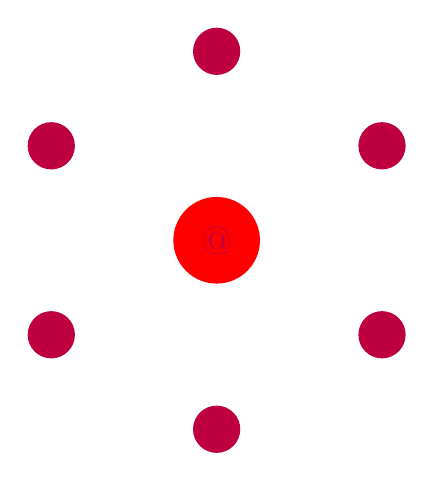
\begin{tikzpicture}[scale=1.0]
\fill[red] (0,0) circle (0.55);
\node[color=purple] at (0,0) {\Large @};

\fill[purple] (0,2.4) circle (0.30);
\fill[purple] (2.1,1.2) circle (0.30);
\fill[purple] (2.1,-1.2) circle (0.30);
\fill[purple] (0,-2.4) circle (0.30);
\fill[purple] (-2.1,-1.2) circle (0.30);
\fill[purple] (-2.1,1.2) circle (0.30);
\end{tikzpicture}
\end{figure}

スライド自体は抽象的である。まだ問いには答えていない。ただ問題の幾何学を固定しているだけだ。もしメッセージが中心から外へ配布できるのなら、演じることの必然性はどこにあるのか。講義の次の一手は、それに比喩ではなく、効果によって答えることである。

\section{人間性が情報をインスピレーションへ変える}

講師は、話には印刷された言葉以上のものを与えられる、と言う。だが、その ``何か余分なもの'' は自動的には起こらない。それは考え抜かれ、注ぎ込まれ、育てられ、勝ち取られなければならない。この insistence は重要である。人間的な層は、人が舞台に立っているというだけで保証されるものではない。それが効力を持つのは、聞き手の内部で起こることを変えるときだけである。

その変化はどのような姿をとるのか。講義は、聴衆自身の想像上の声を通して答える。
\begin{itemize}
\item ``この人は信頼できる。''
\item ``どの文も面白く聞こえる。''
\item ``あなたの声にそれが聞こえるし、顔にもそれが見える。''
\item ``あの言葉へのあの手振りの強調で、いま分かった。''
\item ``それがどれほどあなたを傷つけたか分かる。''
\item ``その情熱はうつる。''
\item ``その目には、なんという決意があるのだろう。''
\item ``この人のチームに加わりたい。''
\end{itemize}

この並びは、注意深く段取りされている。信頼、関心、強調、共感、興奮、確信、行動は、それぞれ別個の飾りではない。情報が他者の心の中で能動的になる、連続した仕方なのである。

\subsection{Question \& Answer}

\paragraph{Question.} ライブの話が、原稿以上に付け加える ``何か余分なもの'' とは何か。

\paragraph{Answer.} それは私たちの人間性であり、操作的に言えば、同じ情報を聴衆がどう受け取るかを変える、聞こえ、見える層である。話し手の存在が、意味を、感じられ、信じられ、行動へ移されるものへ変えるとき、話はテキスト以上のものになる。

この連鎖全体を、講義は一つの支配的な語に圧縮する。
\begin{equation}
\text{人間性} + \text{情報} \Longrightarrow \text{インスピレーション}.
\end{equation}

\begin{definition}
この講義において、\emph{inspiration} とは、新しいアイデアをただ記録され忘れ去られるものにするのではなく、心にそれをどう扱うべきかを告げる力のことである。
\end{definition}

ここから、すっきりとした対比が得られる。
\begin{align}
\text{ふつうのアイデア} &\Longrightarrow \text{しまい込まれる}, \\
\text{インスピレーション} &\Longrightarrow \text{注意が目覚める}.
\end{align}

この移行こそが、講義の本当の蝶番である。私たちは、話すことと書くことの差をめぐる社会的な問いから始めた。だが今や、機能的な定義へと導かれている。inspiration が、それが何をするかによって定義された以上、講師はようやく、話し手の側でそれを左右する変数は何かを問うことができる。

\section{考えるべき二つの大きなこと}

この地点で講義は、効果から方法へと向きを変える。もし inspiration が目標なのだとしたら、話の準備において、私たちが取り組むべき主要なことは何か。答えは驚くほど経済的である。考えるべき大きなことは二つある。声をどう使っているか。そして身体をどう使っているかである。

この分解は重要である。なぜなら、議論が一般論へと溶けてしまうのを防ぐからだ。講義は、``カリスマ的であれ'' とか ``情熱的であれ'' とは言わない。場を二つの制御可能な変数へと還元し、それらを一つずつ検討していく。

\subsection{Question \& Answer}

\paragraph{Question.} 話の準備をするとき、実際に最適化すべき二つの大きなものは何か。

\paragraph{Answer.} 最適化すべきなのは二つである。声。なぜなら、それが意味の聞こえ方を形づくるからである。身体。なぜなら、それが自信、強調、落ち着きの見え方を形づくるからである。

この構造的な分岐は、次のように書ける。
\begin{equation}
\text{話の準備} \Longrightarrow \text{声} + \text{身体}.
\end{equation}

対応するスライドは、これをラベル付きの定理としてではなく、分岐の形として示している。上に大きな問いがあり、中ほどに分岐点があり、その下に対照的な道筋がある。

\begin{figure}[h]
\centering

\includegraphics[width=0.68\textwidth]{how_to_speak_with_meaning_figure_03.png}
\end{figure}

\begin{figure}[h]
\centering
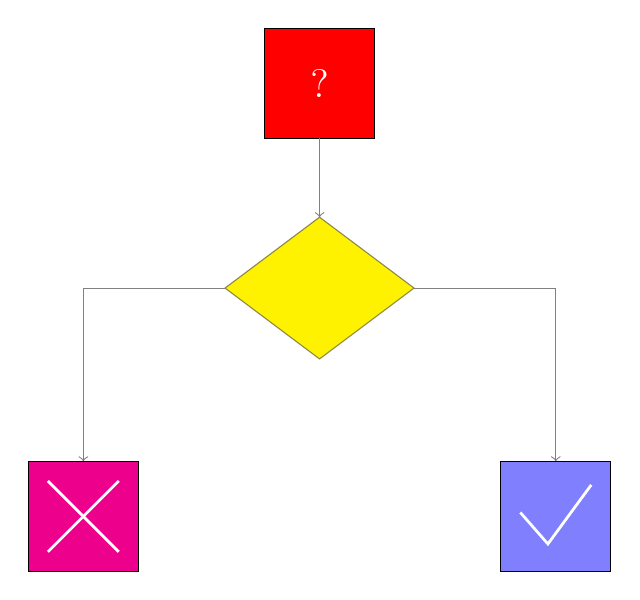
\begin{tikzpicture}[scale=1.0]
\draw[fill=red] (-0.7,2.4) rectangle (0.7,3.8);
\node[color=white] at (0,3.1) {\Large ?};

\draw[->, gray] (0,2.4) -- (0,1.4);

\draw[fill=yellow, draw=yellow!50!black] (0,1.4) -- (-1.2,0.5) -- (0,-0.4) -- (1.2,0.5) -- cycle;

\draw[gray] (-1.2,0.5) -- (-3.0,0.5) -- (-3.0,-1.0);
\draw[gray] (1.2,0.5) -- (3.0,0.5) -- (3.0,-1.0);
\draw[->, gray] (-3.0,-1.0) -- (-3.0,-1.7);
\draw[->, gray] (3.0,-1.0) -- (3.0,-1.7);

\draw[fill=magenta] (-3.7,-3.1) rectangle (-2.3,-1.7);
\draw[white, line width=1pt] (-3.45,-2.85) -- (-2.55,-1.95);
\draw[white, line width=1pt] (-3.45,-1.95) -- (-2.55,-2.85);

\draw[fill=blue!50] (2.3,-3.1) rectangle (3.7,-1.7);
\draw[white, line width=1pt] (2.55,-2.35) -- (2.9,-2.75) -- (3.45,-2.0);
\end{tikzpicture}
\end{figure}

この画像は transcript より抽象的である。transcript のほうが、その構造を二つの枝に名前を与えることで解きほぐしてくれる。その順序は紙面にも残しておく価値がある。まず分岐の形を見る。そしてそのあと、それを何が満たしているのかを教えられるのである。

\section{声: 意味に従う変化}

講師は、最初の枝である声に、規則によってではなく、実例によって入っていく。私たちは George Monbiot の冒頭一分へと送られ、どのようにその効果が生まれているかを告げられる前に、まずその効果そのものに気づくよう促される。これは教育上重要である。私たちは、まず現象を聞く。そのあとでようやく、その機構に名前を与える。

Monbiot の逸話の正確な細部そのものは、ここでの要点ではないし、そのあたりの transcript にはところどころ乱れもある。重要なのは、その周囲にある安定した教訓である。彼の声は、一つ一つの語に意味を加えている。聴衆が彼の世界へ引き込まれるのは、単に言葉がよいからではない。届け方が、それらの言葉のあいだに差異をつくっているからである。ある句は広がり、ある句は引き締まり、ある考えは着地することを許される。私たちは、単なる順列ではなく、構造を聞き取るのである。

\subsection{Question \& Answer}

\paragraph{Question.} どうすれば、言葉をただ正しいだけでなく、生きているように感じさせられるのか。

\paragraph{Answer.} 話し方に変化をつくり、その変化を意味に応答させることである。よい vocal variety は装飾ではない。意味論的なものである。それは、どこに重みがあるのかを聴衆に告げる。

したがって、支配的な規則は次のようになる。
\begin{equation}
\text{話し方の変化} \Longrightarrow \text{意味が聞こえる形になる}.
\end{equation}

講義はそのあと、反例によってこの点を鋭くする。すべての話が、この余分な人間的層を備えているわけではない。自らを平板にしてしまう話もある。どの文も同じ輪郭、同じ小さな上がり下がり、同じ速さ、同じ圧で与えられる。すると聴衆には、誤った信号が与えられる。
\begin{equation}
\text{どの文も同じように聞こえる} \Longrightarrow \text{どの部分も他より重要に見えなくなる}.
\end{equation}

だからこそ講義は、そのような話し方を、悪い意味での催眠になぞらえる。それは聴衆を眠らせてしまう。問題は、単なる退屈ではない。構造上の問題なのである。均質な声は、議論の階層性を否認してしまう。

\section{声が動けるように原稿に印をつける}

この診断が与えられると、講義は手続き的になる。原稿のある話なら、声の変化が自然に現れるのを受け身で待っていてはならない、と言われる。変化をページの上にあらかじめ組み込むべきなのである。実質的には、原稿の上に、届け方のための記譜法を書き込むのだ。

ここは、この講義の中でも最も力強い場面の一つである。なぜなら、曖昧な助言を、実際に使える algorithm に置き換えるからである。私たちは局所から始める。一文ごとに。そして次に、より大きな単位へ移る。段落ごとにである。

\subsection{Question \& Answer}

\paragraph{Question.} 原稿のある話では、どう印をつければ、意味に応じて声が変わり、単調へ滑り落ちずにすむのか。

\paragraph{Answer.} まず各文で最も重要な二語か三語に下線を引く。つぎに各段落で本当に重要な一語を見つけ、それには二重線を引く。そのあと、局所的な特殊効果のために特別な記号を加える。遊び心、問い、冗談、そして主たる aha moment のための印である。

講義の記法は、まず文レベルと段落レベルの強調の区別から始まる。
\begin{align}
\text{文} &\mapsto \underline{\text{重要な語}}, \\
\text{段落} &\mapsto \underline{\underline{\text{その段落を支配する一語}}}.
\end{align}

視覚的なスライドは、まさにこの構造を記録している。テキストのようなブロックがあり、その内部で、強調のための位置が選ばれている。

\begin{figure}[h]
\centering

\includegraphics[width=0.63\textwidth]{how_to_speak_with_meaning_figure_04.png}
\end{figure}

\begin{figure}[h]
\centering
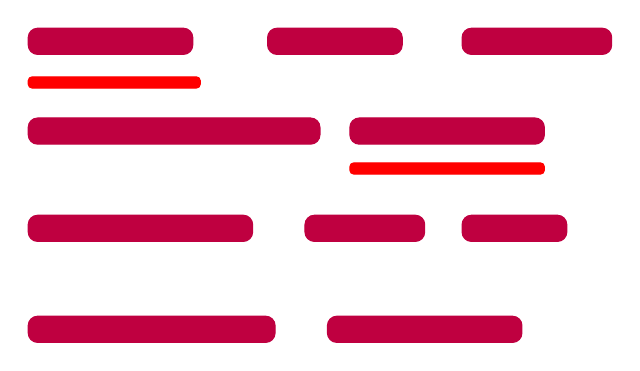
\begin{tikzpicture}[scale=0.95]
\draw[fill=purple, draw=purple, rounded corners=0.12cm] (-3.1,2.4) rectangle (-0.9,2.75);
\draw[fill=purple, draw=purple, rounded corners=0.12cm] (0.1,2.4) rectangle (1.9,2.75);
\draw[fill=purple, draw=purple, rounded corners=0.12cm] (2.7,2.4) rectangle (4.7,2.75);

\draw[fill=red, draw=red, rounded corners=0.05cm] (-3.1,1.95) rectangle (-0.8,2.1);

\draw[fill=purple, draw=purple, rounded corners=0.12cm] (-3.1,1.2) rectangle (0.8,1.55);
\draw[fill=purple, draw=purple, rounded corners=0.12cm] (1.2,1.2) rectangle (3.8,1.55);

\draw[fill=red, draw=red, rounded corners=0.05cm] (1.2,0.8) rectangle (3.8,0.95);

\draw[fill=purple, draw=purple, rounded corners=0.12cm] (-3.1,-0.1) rectangle (-0.1,0.25);
\draw[fill=purple, draw=purple, rounded corners=0.12cm] (0.6,-0.1) rectangle (2.2,0.25);
\draw[fill=purple, draw=purple, rounded corners=0.12cm] (2.7,-0.1) rectangle (4.1,0.25);

\draw[fill=purple, draw=purple, rounded corners=0.12cm] (-3.1,-1.45) rectangle (0.2,-1.1);
\draw[fill=purple, draw=purple, rounded corners=0.12cm] (0.9,-1.45) rectangle (3.5,-1.1);
\end{tikzpicture}
\end{figure}

そのうえで講義は、第二の記号の族を加える。
\begin{align}
\text{疑問符} &\mapsto \text{強調}, \\
\text{遊びのある箇所} &\mapsto \text{波線の下線}, \\
\text{aha moment} &\mapsto \text{その前の黒いしみ}, \\
\text{冗談やおかしな話} &\mapsto \text{その上のピンクの点}.
\end{align}

これらの印は飾りではない。指示なのである。それらは声に、何をするべきかを告げる。
\begin{equation}
\text{原稿上の印} \Longrightarrow \text{それに対応する声の変化}.
\end{equation}

\paragraph{Worked procedure.} 講義の方法は、原稿から発話への制御された移行として次のように書ける。
\begin{enumerate}
\item 原稿を文ごとに読み、その文の局所的な重みを担う少数の語に下線を引く。
\item 一段階上がって、各段落の動きを支配するただ一つの語を選び、それに二重線を引く。
\item 問い、遊びのある部分、冗談、そして主たる aha moment に、それぞれ独自の視覚的記号をつける。
\item もう一度読み、今度は間、速さ、柔らかさ、強調を、その印に応答させる。
\item さらにもう一度読み、今度は各部分の感情状態を声に入れる。
\end{enumerate}

この最後の段階が、手続き全体を機械的なものにしない。講義は明示的に、話のさまざまな部分に結びついている感情、すなわち、どの箇所が情熱、怒り、笑い、困惑を呼び起こすのかを思い出せ、と求める。そうしてはじめて、この印は単なるタイポグラフィ以上のものになる。検査は経験的である。友人に試してみるか、録音して、目を閉じて聞き返してみるのである。

\section{身体: 姿勢、動き、静止}

声に方法が与えられてはじめて、講義は身体へと向きを変える。ここでもまた、失敗の型から始まる。ある話し手たちは、頭を運ぶためだけに存在する身体を連れて舞台に現れるかのように見える。だが舞台に立つと、その身体は不確かになる。手は脇に固定され、重心は揺れ、動きは意図を失う。

講師の最初の処方は、驚くほど単純である。まっすぐ立つこと。両足に等しく体重を乗せること。足は数インチ離しておくこと。問題は、芝居がかった堂々さではない。身体の残りすべてが読めるようになるための、安定した土台である。

\subsection{Question \& Answer}

\paragraph{Question.} 話し手はじっと立つべきか、それとも舞台を動き回るべきか。

\paragraph{Answer.} どちらでもよい。だが、静止はいつでも使える状態でなければならず、動きには目的がなければならない。聴衆が見るべきなのは、リズムと制御であって、内面の不快が外へ漏れ出すさまではない。

見えているスライドは、この鍵となる関係を象徴的に与えている。
\begin{equation}
\text{左足にかかる重さ} = \text{右足にかかる重さ}.
\end{equation}

\begin{figure}[h]
\centering

\includegraphics[width=0.56\textwidth]{how_to_speak_with_meaning_figure_05.png}
\end{figure}

この式は、慎重な再構成である。等号はフレーム内にはっきり見えており、左右の変数の解釈は transcript によって補われている。しかしこの再構成は、講義の要点に忠実である。身体のバランスは、落ち着いた力の第一条件なのだ。

その土台が安定すれば、上半身は動いてよい。手と腕は、語られている内容を自然に強調してよい。よい姿勢は助けになる。猫背は信号を弱める。そこから講義は、姿勢からリズムへと広がる。
\begin{equation}
\text{目的ある動き} + \text{静止の瞬間} \Longrightarrow \text{力ある舞台のリズム}.
\end{equation}

それに対応する警告も同じく鋭い。
\begin{equation}
\text{絶え間ない歩き回りや揺れ} \Longrightarrow \text{聴衆に見える不快さ}.
\end{equation}

\paragraph{Practical rule.} 身体の側の algorithm は、短く具体的である。
\begin{enumerate}
\item 安定した土台をつくる。
\item 身振りは不安からではなく、内容から生じさせる。
\item 動きが思考や強調を助けるときに動く。
\item 重要な点を着地させる必要があるときには止まる。
\item 反復的な揺れは取り除く。それは意味よりも神経質さを宣伝してしまうからである。
\end{enumerate}

ここでの ``calm power'' という講義の言葉は的確である。私たちは身体を凍らせたいのではない。読めるものにしたいのである。

\section{唯一の型はなく、あるのは無理のない自信だけ}

この時点で講義は、欠かせない修正の動きを見せる。具体的な thumb rule を与えたあとで、それをよい話し方の一律の模型へ変えることを拒むのだ。座って話す人もいる。非常に活発に動く人もいる。ほとんど完全に静止して立つ人もいる。講師が Dame Stephanie Shirley、Oliver Sacks、Clifford Stoll に言及するのは、まさに模倣への誘惑を断ち切るためである。

これは先ほどの助言からの撤退ではない。その完成である。講義の規則は、同じ話し方を量産するためのものではない。避けうる干渉を取り除くためのものなのである。そうした干渉が消えたときにはじめて、異なる舞台スタイルが、気を散らすものになることなく、それぞれに花開くことができる。

したがって最後の基準は、ある正典的な話し手に似ているかどうかではない。舞台の占め方が、自分自身を快適で自信のあるものに感じさせるかどうか、そして、そのことがアイデアをきれいに通過させるかどうかである。講義は、この検査を具体的に保っている。少人数の聴衆の前でリハーサルするか、自分の姿を見返して、身体言語がメッセージを助けているのか、それとも妨げているのかを問うのである。

そしてここで、この話は静かにその冒頭の論理へ戻る。届け方全体の目的は、アイデアを力を伴って到着させることにある。身体は、パフォーマンスを飾るためにあるのではない。それは意味を運ぶ装置の一部なのだ。

\section{まとめ}

この講義は、制御された議論として展開する。私たちはまず、ひとつの挑戦から始める。言葉がすでにページ上にあるのなら、なぜそもそもそれを声に出して語るのか。答えは、ライブの発話が、人間的な層を加え、そのことによって情報をインスピレーションへと変えうる、というものである。いったんそれが理解されれば、講義は準備を、私たちが実際に取り組める二つの変数へと還元する。声と身体である。

声の側では、中心原理は、変化が意味に従わなければならない、ということだ。声は階層を刻むべきであって、それを平板にしてはならない。だからこそ講義は、原稿に注記を施す明示的な方法を与えてくれる。重要な語に下線を引き、段落を支配する語には二重の印をつけ、問い、遊び、ユーモア、そして主たる aha moment には局所的な記号を加えるのである。身体の側では、講義はまずバランスから始まり、ついで身振り、動き、静止へと広がっていくが、つねに、動きは不安を漏らすためではなく、強調に奉仕するものでなければならないと insist している。

したがって、この章は講義と同じところで終わる。模倣すべき単一のパフォーマンス様式などない。私たちが求めているのは、アイデアが、明晰さと確信、そして紛れもない人間的な存在感を伴って届いていくことを許すような、声と身体なのである。